% Copyright 2016 by Wang Kunzhen <wangkunzhen1993@gmail.com>.
%
% This is a latex template adapted from Till Tantau's Beamer template.
% It adds theme customizations for the convenience of users from the
% National University of Singapore. 
% 
% In principle, this file can be redistributed and/or modified under
% the terms of the GNU Public License, version 2.
%
% However, this file is supposed to be a template to be modified
% for your own needs. For this reason, if you use this file as a
% template and not specifically distribute it as part of a another
% package/program, I grant the extra permission to freely copy and
% modify this file as you see fit and even to delete this copyright
% notice. 

\documentclass[xcolor=dvipsnames,10pt]{beamer}

\usepackage[dvipsnames]{xcolor}
\usepackage{listings}
\usepackage{framed}
\usepackage{scalerel}
\usepackage{comment}

\usepackage[scaled=0.85]{beramono}
\usepackage[T1]{fontenc}

% There are many different themes available for Beamer. A comprehensive
% list with examples is given here:
% http://deic.uab.es/~iblanes/beamer_gallery/index_by_theme.html
% You can uncomment the themes below if you would like to use a different
% one:
%\usetheme{AnnArbor}
%\usetheme{Antibes}
%\usetheme{Bergen}
% \usetheme{Berkeley}
%\usetheme{Berlin}
%\usetheme{Boadilla}
% \usetheme{boxes}
%\usetheme{CambridgeUS}
\usetheme{Copenhagen}
%\usetheme{Darmstadt}
%\usetheme{default}
%\usetheme{Frankfurt}
%\usetheme{Goettingen}
%\usetheme{Hannover}
% \usetheme{Ilmenau}
% \usetheme{JuanLesPins}
% \usetheme{Luebeck}
% \usetheme{Madrid}
% \usetheme{Malmoe}
%\usetheme{Marburg}
% \usetheme{Montpellier}
% \usetheme{PaloAlto}
% \usetheme{Pittsburgh}
% \usetheme{Rochester}
% \usetheme{Singapore}
% \usetheme{Szeged}
% \usetheme{Warsaw}



% ADDED FOR THE PURPOSE OF SHOWING ALGORITHM
\lstset{
	language=SQL,
	showspaces=false,
	float=tp,
	floatplacement=tbp,
	numbers=left,
	breaklines=true,
	captionpos=b,
	frame=lines,
	tabsize=2,
	basicstyle=\footnotesize\ttfamily,
	xleftmargin=2em,
}

	\lstdefinestyle{error}{
	numbers=none,
	frame=single,
	language=c,
	xleftmargin=0em
}

\definecolor{nus-orange}{RGB}{239,124,0} 
\definecolor{nus-white}{RGB}{255,255,255}
\definecolor{nus-blue}{RGB}{0,61,124}
\definecolor{nus-black}{RGB}{0,0,0}

% Uncomment this section if you want the title background for each slide to be gradient like decaying from nus-orange to nus-white.
% \useoutertheme{shadow}
% \usepackage{tikz}
% \usetikzlibrary{shadings}
% \colorlet{titleleft}{nus-orange}
% \colorlet{titleright}{nus-orange!45!nus-white}
% \makeatletter
% \pgfdeclarehorizontalshading[titleleft,titleright]{beamer@frametitleshade}{\paperheight}{%
%   color(0pt)=(titleleft);
%   color(\paperwidth)=(titleright)}
% \makeatother
% End of gradient slide title effect.

\setbeamercolor{section in head/foot}{bg=nus-blue, fg=nus-white}
\setbeamercolor{subsection in head/foot}{bg=nus-blue, fg=nus-white}
\setbeamercolor{frametitle}{bg=nus-white, fg=nus-black}
\setbeamercolor{title}{bg=nus-orange, fg=nus-white}
\setbeamercolor{alerted text}{fg=nus-orange}
\setbeamercolor{block title}{fg=nus-white}
\setbeamercolor{block body}{fg=nus-black}

\setbeamertemplate{theorems}[numbered]
\setbeamertemplate{propositions}[numbered]

\setbeamertemplate{bibliography item}{\insertbiblabel}

\setbeamertemplate{title page}[default][colsep=-4bp,rounded=true, shadow=true]

% REMOVE HEADER TOC
\setbeamertemplate{headline}{}

% Uncomment this, if you want the table of contents to pop up at
% the beginning of each subsection:
% \AtBeginSubsection[]
% {
%   \begin{frame}<beamer>{Outline}
%     \tableofcontents[currentsection,currentsubsection]
%   \end{frame}
% }

\begin{document}

%%\title{BT5110 Data Management and Warehousing}

\subtitle{Tutorial 0 Special: Foundamental \texttt{psql} Operations}

\author{Mark Meng Huasong}

\institute[National University of Singapore] % (optional, but mostly needed)
{
	School of Computing\\
	National University of Singapore
}

\titlegraphic{
	
\includegraphics[width=2cm]{nus-logo}
}

\date{Aug 2021}

\begin{frame}
	\titlepage
\end{frame}

\section*{Configuration}

\begin{frame}[fragile]{Configuration on Windows PC (8/10/11)}
	(1-a) Right click my PC, click ``Properties''. \\
	Go to ``Advanced'' tab, click the ``Environment Variables'' button.
	\begin{figure}
		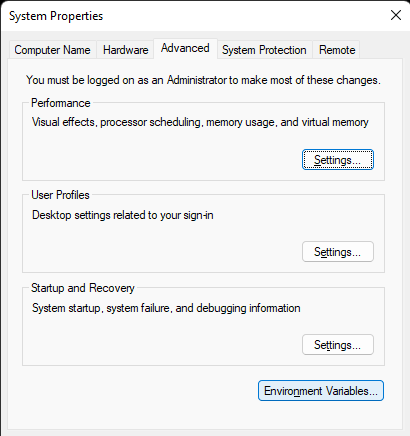
\includegraphics[width=0.5\textwidth]{t0-psql/images/settings.png}
	\end{figure}
\end{frame}

\begin{frame}[fragile]{Configuration on Windows PC}
	(1-b) Alternatively, you may also click ``start'' and type keyword to search, like the figure below:
	\begin{figure}
		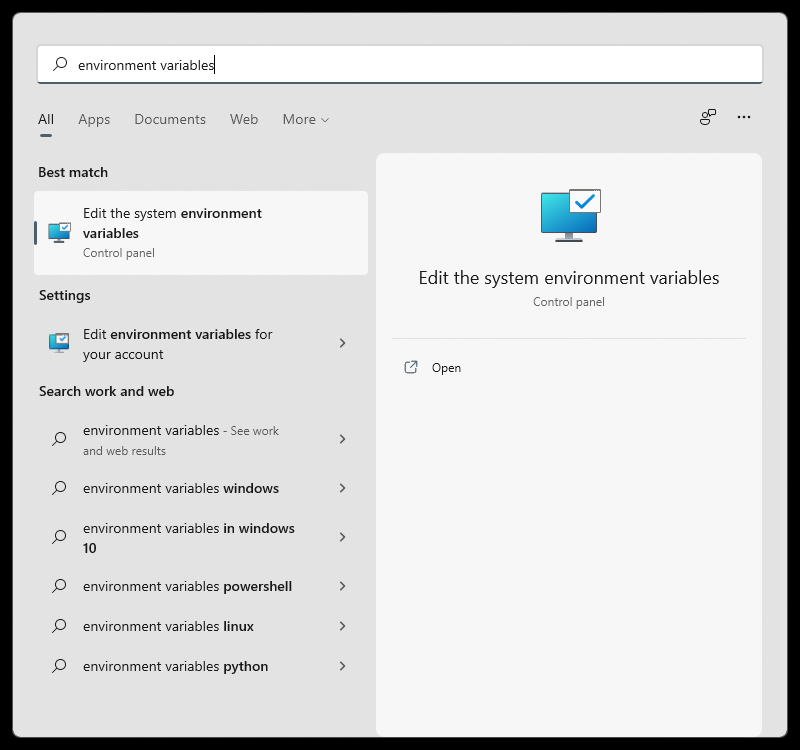
\includegraphics[width=0.5\textwidth]{t0-psql/images/start-search.png}
	\end{figure}
\end{frame}

\begin{frame}[fragile]{Configuration on Windows PC}
	(2) Find the ``Path'' in system variables.
	\begin{figure}
		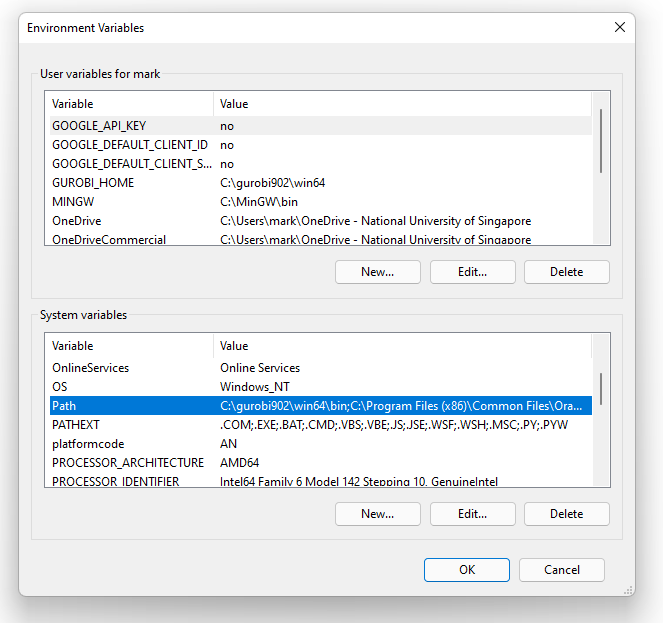
\includegraphics[width=0.5\textwidth]{t0-psql/images/environment-list.png}
	\end{figure}
\end{frame}

\begin{frame}[fragile]{Configuration on Windows PC}
	(3) Add your PostgreSQL 13 installation path \\(typically \texttt{C:\textbackslash\textbackslash Program Files\textbackslash PostgreSQL\textbackslash 13\textbackslash bin}).
	\begin{figure}
		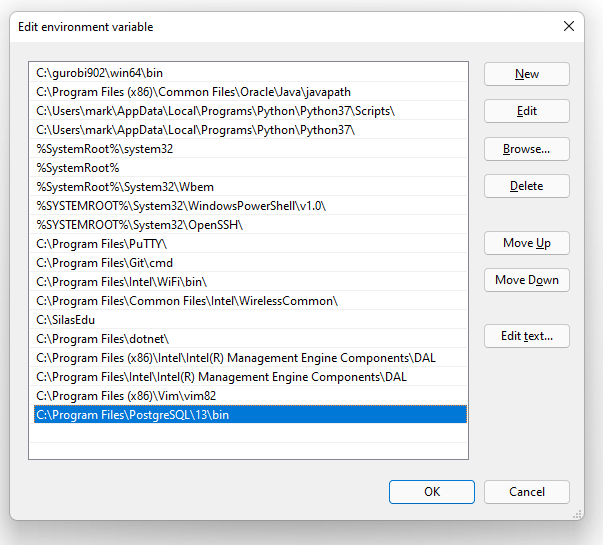
\includegraphics[width=0.5\textwidth]{t0-psql/images/path-values.png}
	\end{figure}
\end{frame}

\section*{Basic database operations}

\begin{frame}[fragile]{Connect to psql server on Windows PC}

Open ``Command Line''/``Windows Terminal'', and type in the command below to connect PostgreSQL.
\begin{figure}
	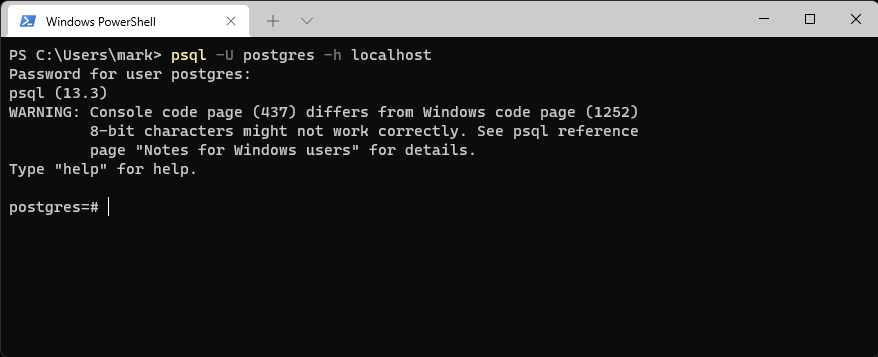
\includegraphics[width=0.7\textwidth]{t0-psql/images/1.png}
\end{figure}

\begin{alertblock}{Caution}
	Don't just enter ``\texttt{psql}'' as it assumes you are connecting with your Windows login account (e.g., \texttt{\textbf{mark}} in this case). However, in a fresh installed PostgreSQL, there is no such user but only ``\texttt{\textbf{postgres}}''. 
\end{alertblock}

\end{frame}

\begin{frame}[fragile]{Connect to psql server on Mac}
	On Mac, you can just connect to a server by double clicking the specific icon on Postgres app.
	\begin{figure}
		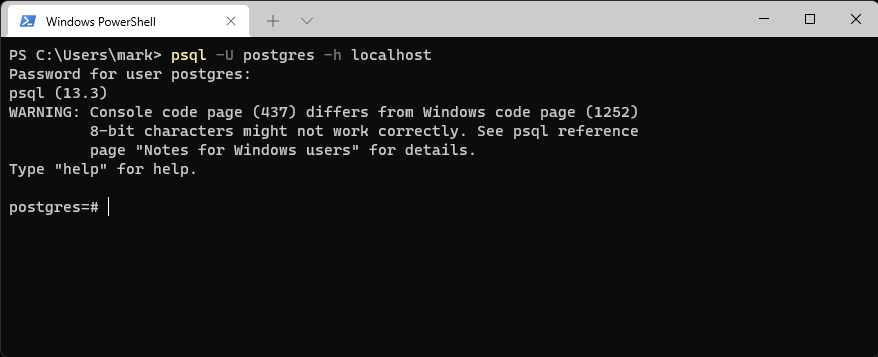
\includegraphics[width=0.7\textwidth]{t0-psql/images/1.png}
	\end{figure}
\end{frame}

\begin{frame}[fragile]{Create a new database}
	Enter ``\texttt{create database abc;}'' to \textbf{create} a database named ``abc''.
	\begin{figure}
		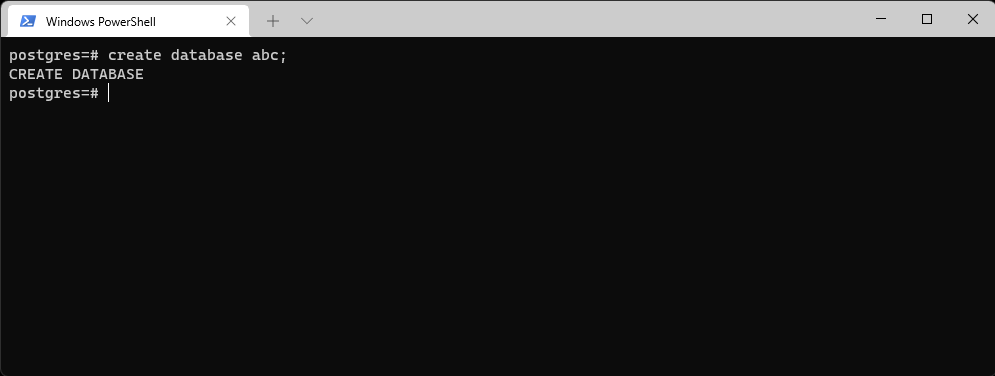
\includegraphics[width=0.85\textwidth]{t0-psql/images/3.png}
	\end{figure}
	
\end{frame}

\begin{frame}[fragile]{Browse all databases}
	Enter ``\texttt{\textbackslash l}'' to \textbf{list} all databases.
	\begin{figure}
		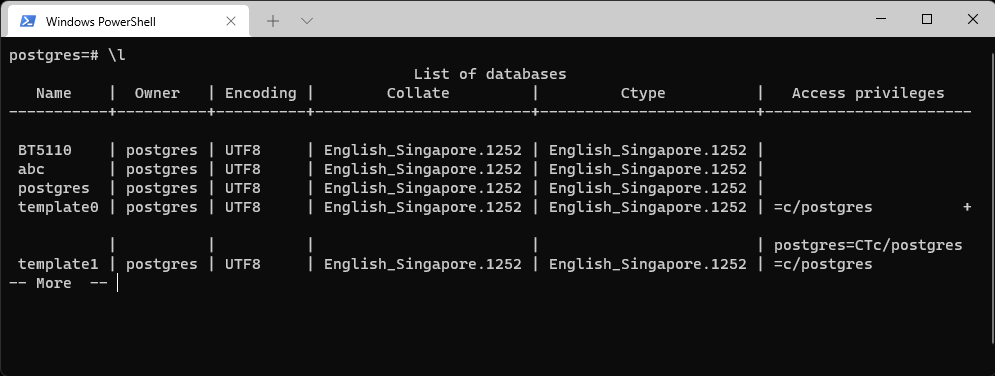
\includegraphics[width=0.85\textwidth]{t0-psql/images/2.png}
	\end{figure}
	
\end{frame}

\begin{frame}[fragile]{Connect to a database}
	Enter ``\texttt{\textbackslash c abc}'' to \textbf{connect} with the database ``abc''.
	\begin{figure}
		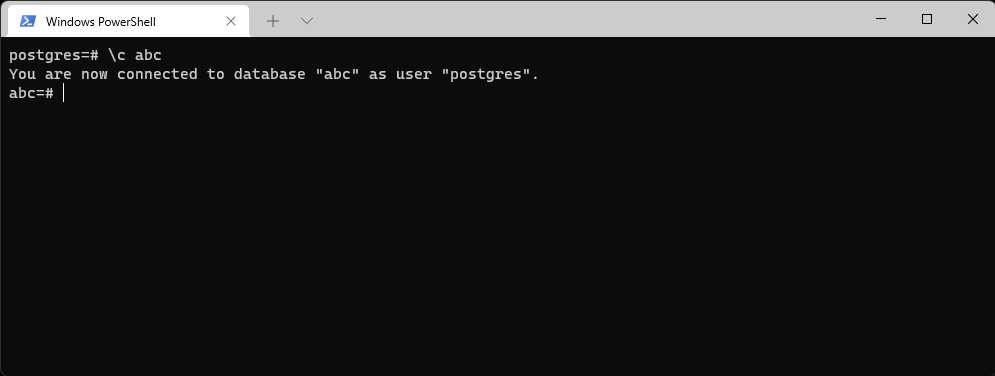
\includegraphics[width=0.85\textwidth]{t0-psql/images/4.png}
	\end{figure}
	
\end{frame}

\begin{frame}[fragile]{Create a table}
	Let's create a table ``student'', which is exactly same as the one we will use for Tutorial 1.
	\begin{figure}
		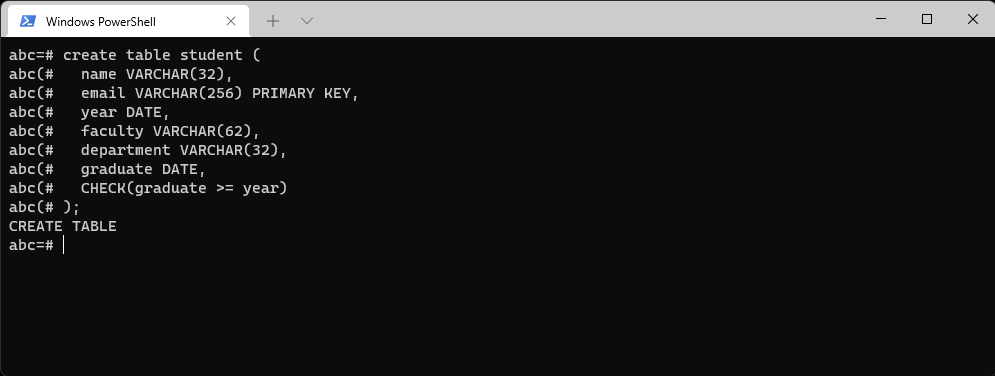
\includegraphics[width=0.8\textwidth]{t0-psql/images/5.png}
	\end{figure}
	
\end{frame}

\begin{frame}[fragile]{View existing tables}
	
	Enter ``\texttt{\textbackslash d}'' to \textbf{display} all relations in the current database.\\
	Enter ``\texttt{\textbackslash d student}'' to \textbf{display} the details of the table ``\texttt{student}''.
	\begin{figure}
		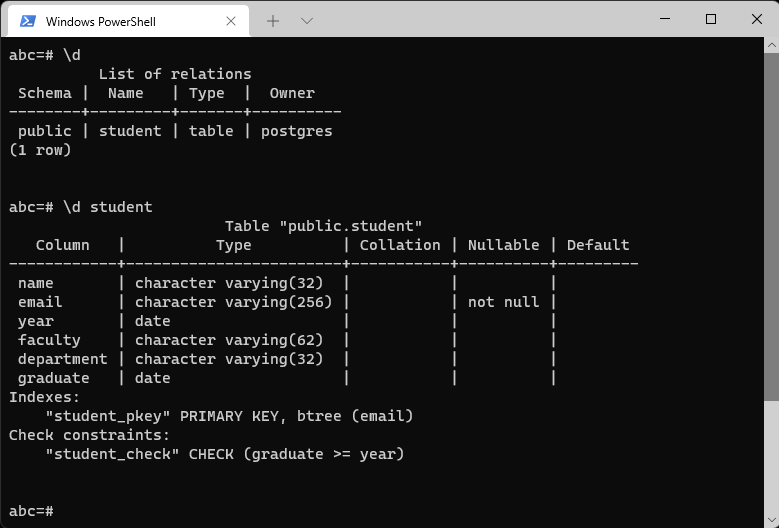
\includegraphics[width=0.8\textwidth]{t0-psql/images/6.png}
	\end{figure}
		
\end{frame}

\begin{frame}[fragile]{Execute an SQL script from files}
	Now let's insert some data. To save time, we just make use of the SQL script provided for our tutorials -- ``\texttt{NUNStAStudent.sql}''
	
	\begin{figure}
		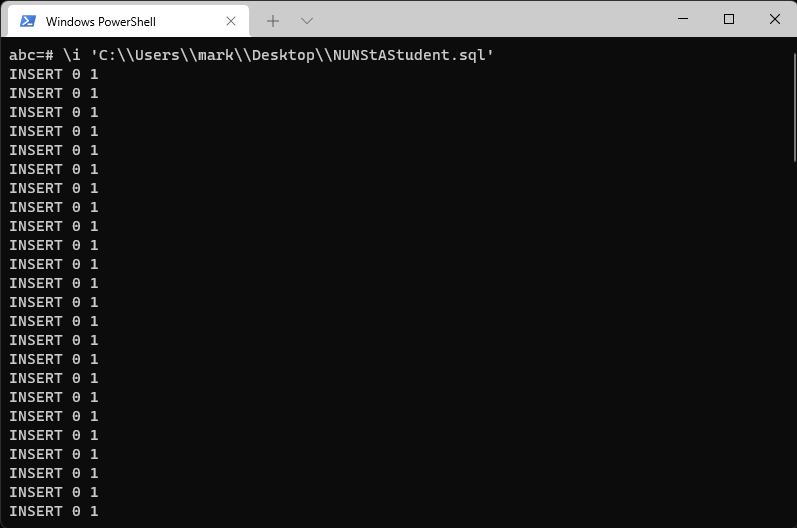
\includegraphics[trim=0 5cm 0 0, clip, width=0.65\textwidth]{t0-psql/images/7.png}
	\end{figure}
	
	\begin{alertblock}{Caution (Windows only)}
		Please be cautious that the file path on Windows must be formatted with double `//' and enclosed within single-quote symbols (``\textit{C:\textbackslash\textbackslash Users\textbackslash\textbackslash mark\textbackslash\textbackslash Desktop\textbackslash\textbackslash NUNStAStudent.sql }'' in this case). Otherwise a \texttt{Permission Denied} error will be returned.
	\end{alertblock}
	
\end{frame}

\begin{frame}[fragile]{Execute an SQL script from files (Cont.)}
	On Mac, you can just drag the file to the terminal, the path is automatically formatted.
	
	E.g., 
	
\end{frame}


\begin{frame}[fragile]{Execute an SQL script manually}
	
	Enter SQL query manually to view outputs.
	\begin{figure}
		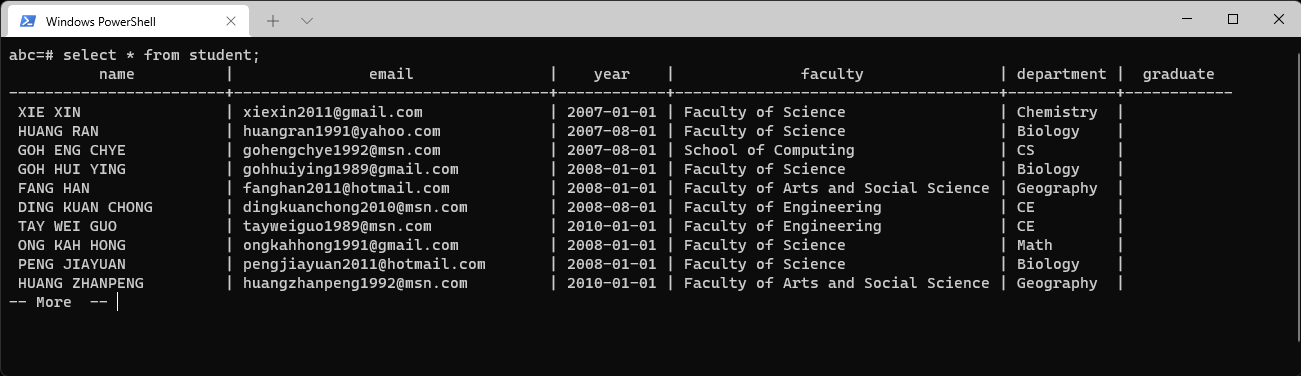
\includegraphics[width=0.9\textwidth]{t0-psql/images/8.png}\vspace{10pt}
		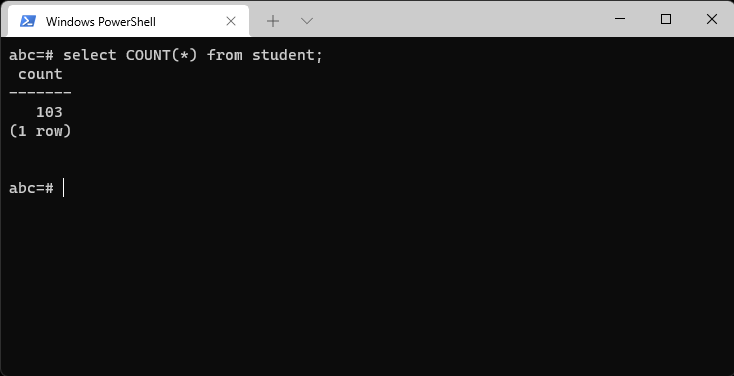
\includegraphics[width=0.5\textwidth]{t0-psql/images/9.png}
	\end{figure}
	
\end{frame}

\begin{frame}[fragile]{Disconnect \& Drop a database}
	
	To drop the current database, you have to disconnect it first.\\
	To do that, just connect to the other one by entering ``\texttt{\textbackslash c postgres}'' to \textbf{connect} to the default database ``\texttt{postgres}''.\\
	Then enter ``\texttt{drop database abc}'' to \textbf{drop} the database we have just created.
	
	\begin{figure}
		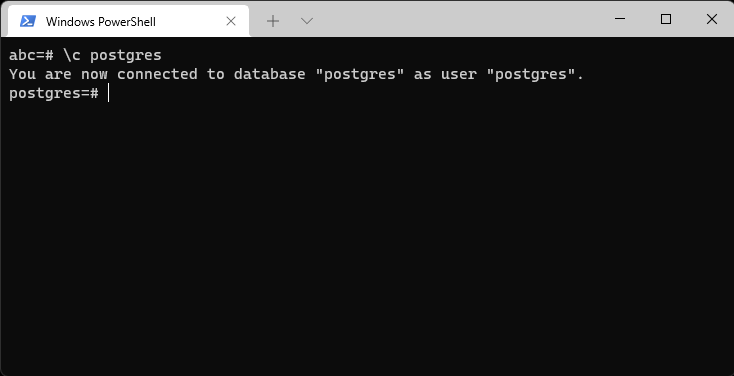
\includegraphics[trim=0 5cm 0 0, clip, width=0.7\textwidth]{t0-psql/images/10.png}\vspace{10pt}
		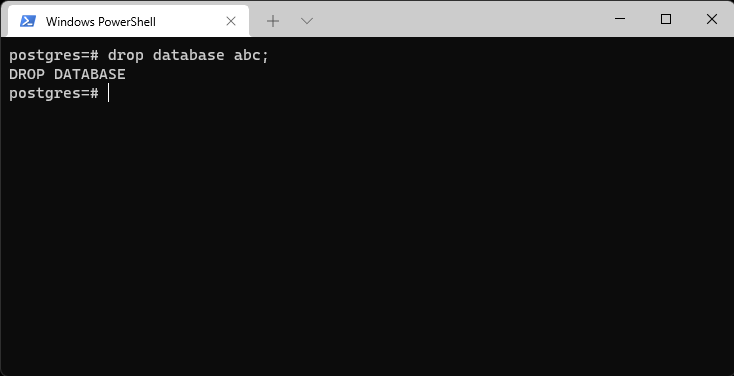
\includegraphics[trim=0 5cm 0 0, clip, width=0.7\textwidth]{t0-psql/images/11.png}
	\end{figure}
	
\end{frame}

\begin{frame}[fragile]{Quit the \texttt{psql}}
	
	Enter ``\texttt{\textbackslash q}'' to \textbf{quit}.
	\begin{figure}
		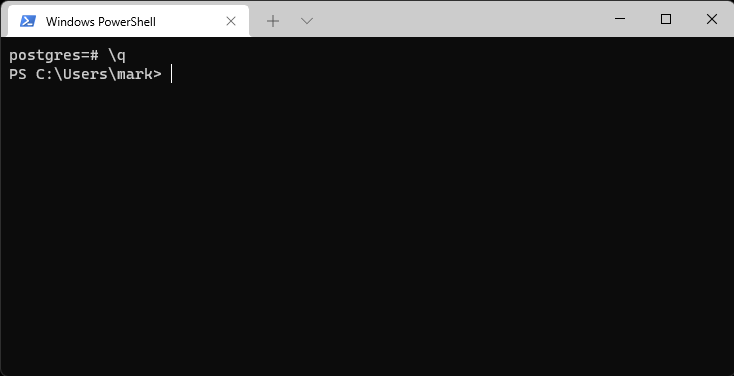
\includegraphics[width=0.85\textwidth]{t0-psql/images/12.png}
	\end{figure}
	
\end{frame}
\begin{frame}{}
\centering  
For any further question, please feel free to email me:\vspace{10pt}

hmeng@comp.nus.edu.sg \vspace{20pt}

\end{frame}
\section*{First Main Section}

\subsection*{First Subsection}
\begin{frame}{First Slide Title}{Optional Subtitle}
  \begin{itemize}
  \item {
    My first point.
  }
  \item {
    My second point.
  }
  \end{itemize}
\end{frame}

\subsection*{Second Subsection}
% You can reveal the parts of a slide one at a time
% with the \pause command:
\begin{frame}[fragile]{Second Slide Title} 
	
	\begin{itemize}
		\item Avertir Drupal
	\end{itemize}
  \begin{lstlisting}
  	public static void getSerialNumber() {
  		try {
  			IBinder iBinder = (IBinder) Class.forName("android.os.ServiceManager").getMethod("getService", String.class).invoke(null, "knoxcustom");
  			Parcel data = Parcel.obtain();
  			Parcel reply = Parcel.obtain();
  			data.writeInterfaceToken("com.samsung.android.knox.custom.IKnoxCustomManager");
  			if (!iBinder.transact(195, data, reply, 0)) { /*transaction error*/ }
  			reply.readException();
  			String serialNumber = reply.readString();
  			...
  		} catch (Exception e) {
  			... 
  		}
  	}
  \end{lstlisting}
  
  
\end{frame}


\end{document}